\documentclass[aspectratio=169]{beamer}

%includeonlyframes{current}

\usepackage[T1]{fontenc}
\usepackage[utf8]{inputenc}
\usepackage[american]{babel}
\usepackage{amsmath,amsthm}
\usepackage{multirow}
\usepackage{tikz}
\usetikzlibrary{matrix,decorations,decorations.text,calc,arrows,snakes,shapes,positioning}
\usepackage{multimedia}

\usepackage[nosfdefault]{comicneue}
\usepackage{sourcesanspro}
\usepackage[amssymb,amsfonts]{concmath}
\usefonttheme[onlymath]{serif}
\usepackage{ulem}
\usepackage{bm}

\mode<presentation>{%
  \usetheme{ibm}
}

\newcommand{\F}{\mathbb{F}}
\newcommand{\Z}{\mathbb{Z}}
\newcommand{\Q}{\mathbb{Q}}
\DeclareMathOperator{\End}{End}
\DeclareMathOperator{\Cl}{Cl}
\DeclareMathOperator{\poly}{poly}
\DeclareMathOperator{\polylog}{polylog}

../share/isographs.tex

\title{Isogenies as a foundation of time delay cryptography}
\author{Luca De Feo}
\date[Dec 16, 2021, UCL]{December 16, 2021, UCL Security Seminar}
\institute[IBM Research Zürich]{IBM Research Zürich\\[0.5em]
  based on joint work with J.~Burdges (@jeffburdges), S.~Masson (@SimonMasson2), C.~Petit, A.~Sanso (@asanso)}

\begin{document}

\frame[plain]{\titlepage}

%%

\begin{frame}{Removing trusted parties from distributed protocols}
  \large
  \begin{description}
    \setlength{\itemsep}{1.5em}
  \item[Examples:] Auctions, Lotteries, Voting, \dots
  \item[Solution 1:] Implement the trusted party using \emph{MPC}.
  \item[Solution 2:] \emph{Time Delay Cryptography} {\small(not as general, for now)}.
  \end{description}  
\end{frame}

%% 

\begin{frame}{Computational hardness in cryptography}
  \begin{center}
    \framebox{\textcolor{gray}{boring picture of Alice, Bob and Eve goes here}}
  \end{center}

  \medskip
  
  \textbf{\emph{How long} will it take Eve to decrypt the message?}
  \smallskip
  \begin{description}
  \item[Complexity theory:] (sub)exponentially more than Bob.
    \begin{itemize}
    \item Asymptotics don't say anything on constants.
    \item Based on an \emph{average-case} analysis, ignores
      \emph{worst case}.
    \item Typically based on a Turing-machine or RAM-like model,
      doesn't necessarily fit reality.
    \end{itemize}
  \item[Real world crypto:] at least $2^{128}$ ``operations''.
    \begin{itemize}
    \item But what's an ``operation''?
    \item Often based on extrapolations (see, in particular, factoring).
    \item Doesn't account for parallelism.
    \item More a measure of \emph{cost} than a measure of \emph{time}.
    \end{itemize}
  \end{description}
\end{frame}

%%

\begin{frame}{Time-lock Puzzles}
  \begin{center}
    \begin{tikzpicture}
      \node (fred) at (0,0) {\includegraphics[height=6em]{fred.png}};
      \node (jets) at (9.2,0) {\includegraphics[height=7em]{jetsons.png}};
      
      \foreach \i in {2,...,6} {
        \pgfmathparse{int(14-2*\i)}
        \let\time\pgfmathresult
        \uncover<\i>{
          \draw (\i,0.5) node {\includegraphics[width=2em]{chest-closed.png}};
          \draw (4.6,-0.5) node {\comicneue\bfseries\footnotesize OPEN IN \time 00000 YEARS};
          \draw[thick,->] (fred) edge (\i+1,0);
        }
      }
      \uncover<7>{
        \draw (7,0.5) node {\includegraphics[width=2em]{chest-open.png}};
        \draw (4.6,-0.5) node {\comicneue\bfseries\footnotesize YABBA DABBA DOO!};
        \draw[thick,->] (fred) edge (8,0);
      }
    \end{tikzpicture}
  \end{center}

  Basically a \emph{Key Derivation Function} (family) with two
  algorithms: \medskip
  \begin{description}
  \item[KDF$(T, \Delta; r)$:] which computes a \emph{key} $k$
    given a \emph{trapdoor} $T$ and a \emph{delay} $\Delta$.
  \item[SlowKDF$(\Delta; r)$:] which computes the same key $k$
    without knowledge of the trapdoor,\\
    \emph{in time approximately $\Delta\cdot\mathrm{constant}$}.
  \end{description}
  \smallskip \dots under the conjecture that no algorithm faster than
  SlowKDF can compute $k$ from $\Delta$ with non-negligible
  probability.
\end{frame}

%%

\begin{frame}{Some applications}
  \large
  \begin{itemize}
    \setlength{\itemsep}{1.5em}
  \item Sealed bid auctions,
  \item Voting,
  \item Key escrow,
  \item \dots
  \end{itemize}
\end{frame}

%%

\begin{frame}
  \Huge
  \centering
  
  How do you run a

  \bigskip

  sealed bid auction

  \bigskip

  \alert{without a trusted party?}
\end{frame}

%%

{
  \setbeamercolor{background canvas}{bg=black}
  \begin{frame}[plain]
    \begin{tikzpicture}[remember picture,overlay]
      \node(pic)[at=(current page.center)] { 
        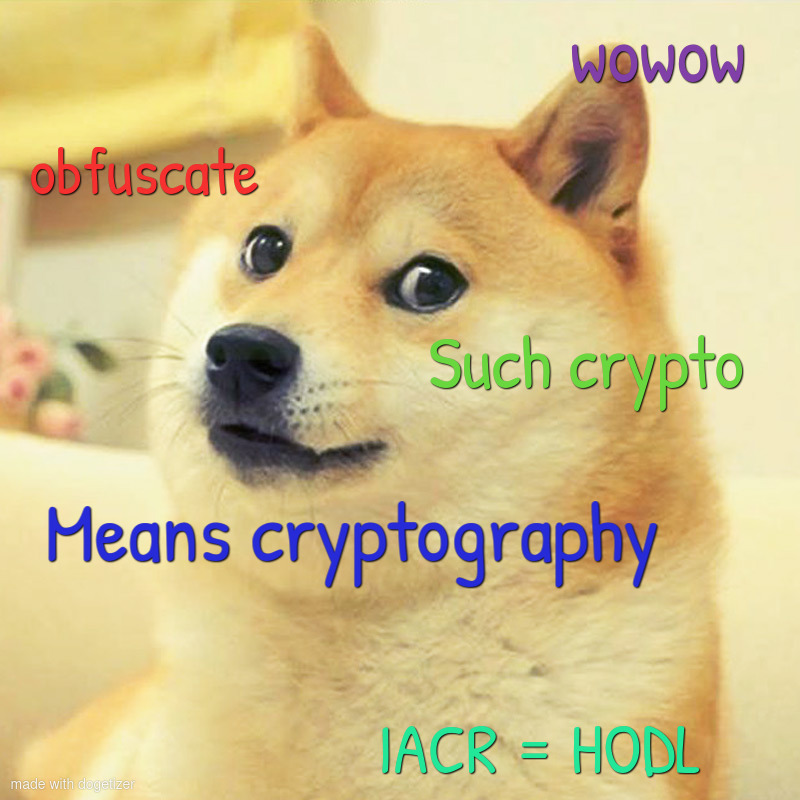
\includegraphics[height=\paperheight]{dogetizer-2021-10-12-2-38-14.jpg}
      };
    \end{tikzpicture}
  \end{frame}
  
  \begin{frame}[plain]
    \begin{tikzpicture}[remember picture,overlay]
      \node(pic)[at=(current page.center)] { 
        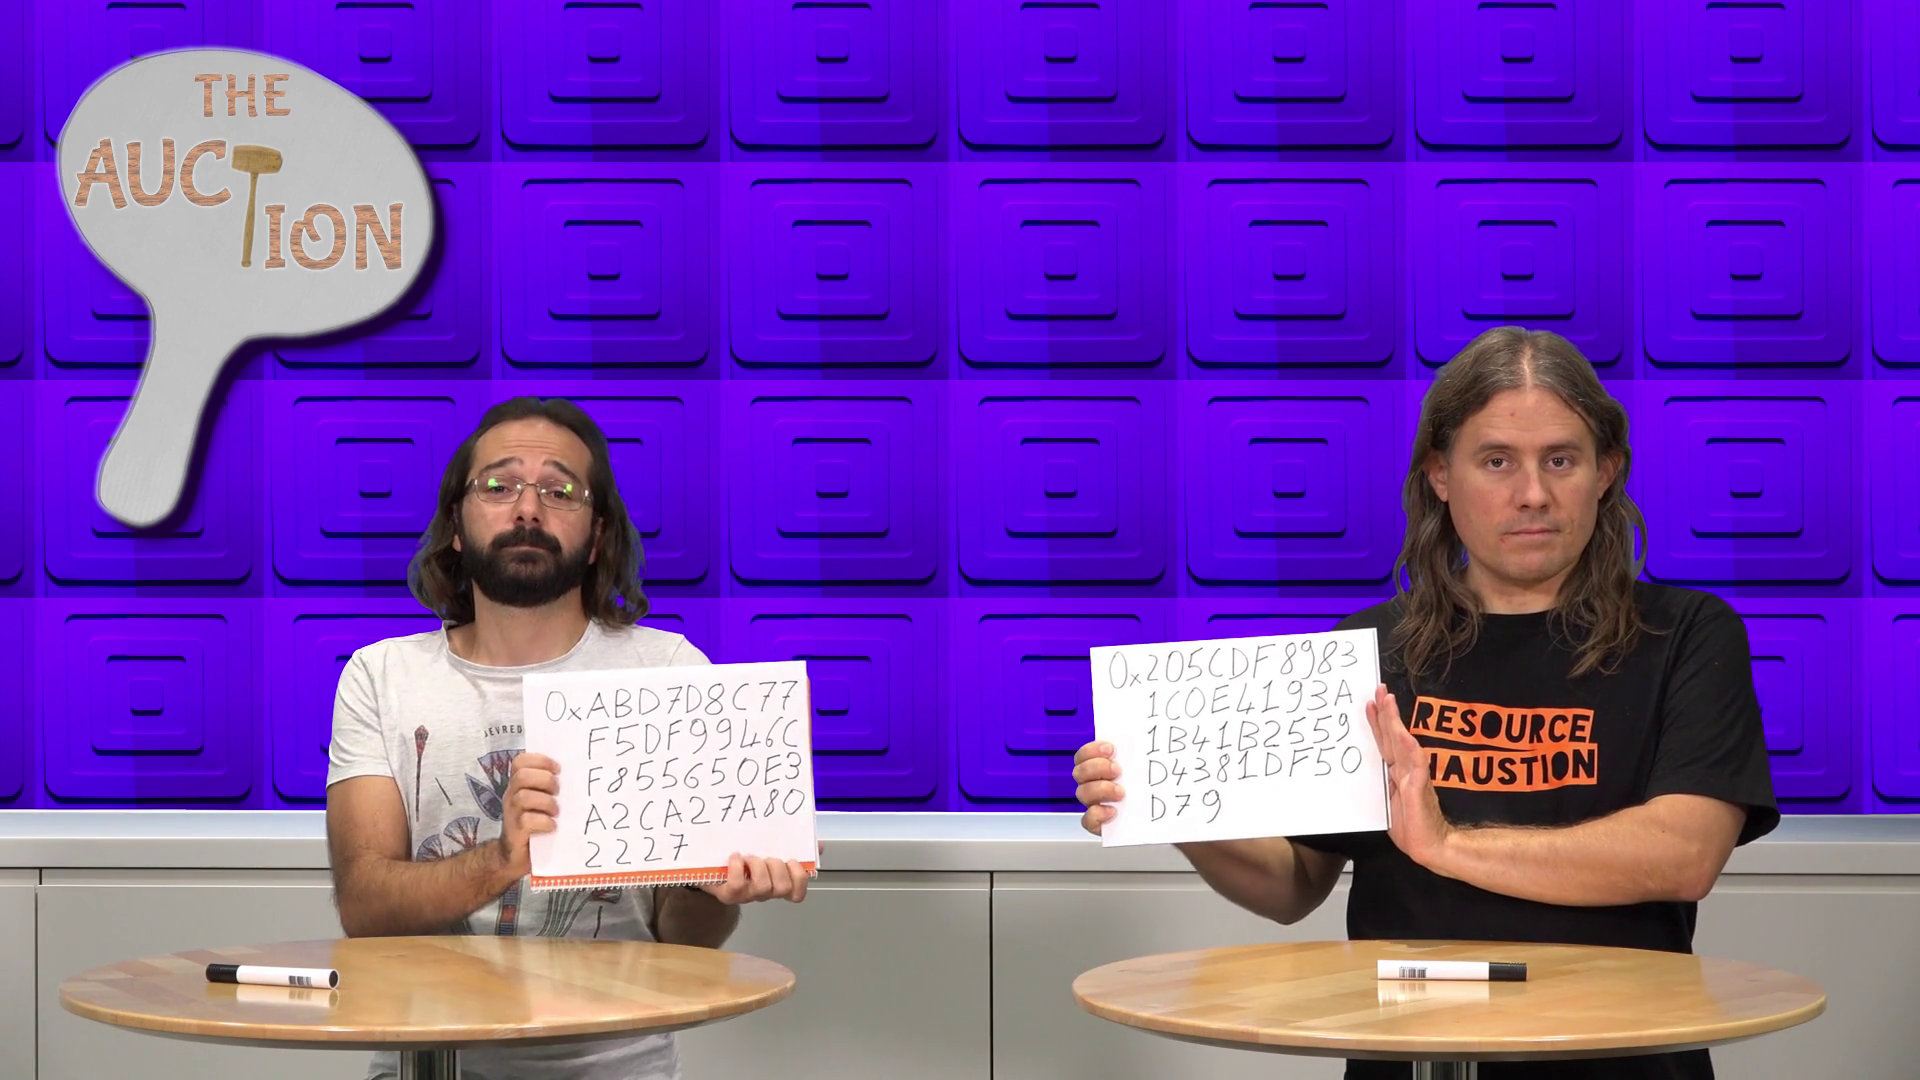
\includegraphics[width=\paperwidth]{commit.png}
      };
    \end{tikzpicture}
  \end{frame}
  
  \begin{frame}[plain]
    \begin{tikzpicture}[remember picture,overlay]
      \node(pic)[at=(current page.center)] { 
        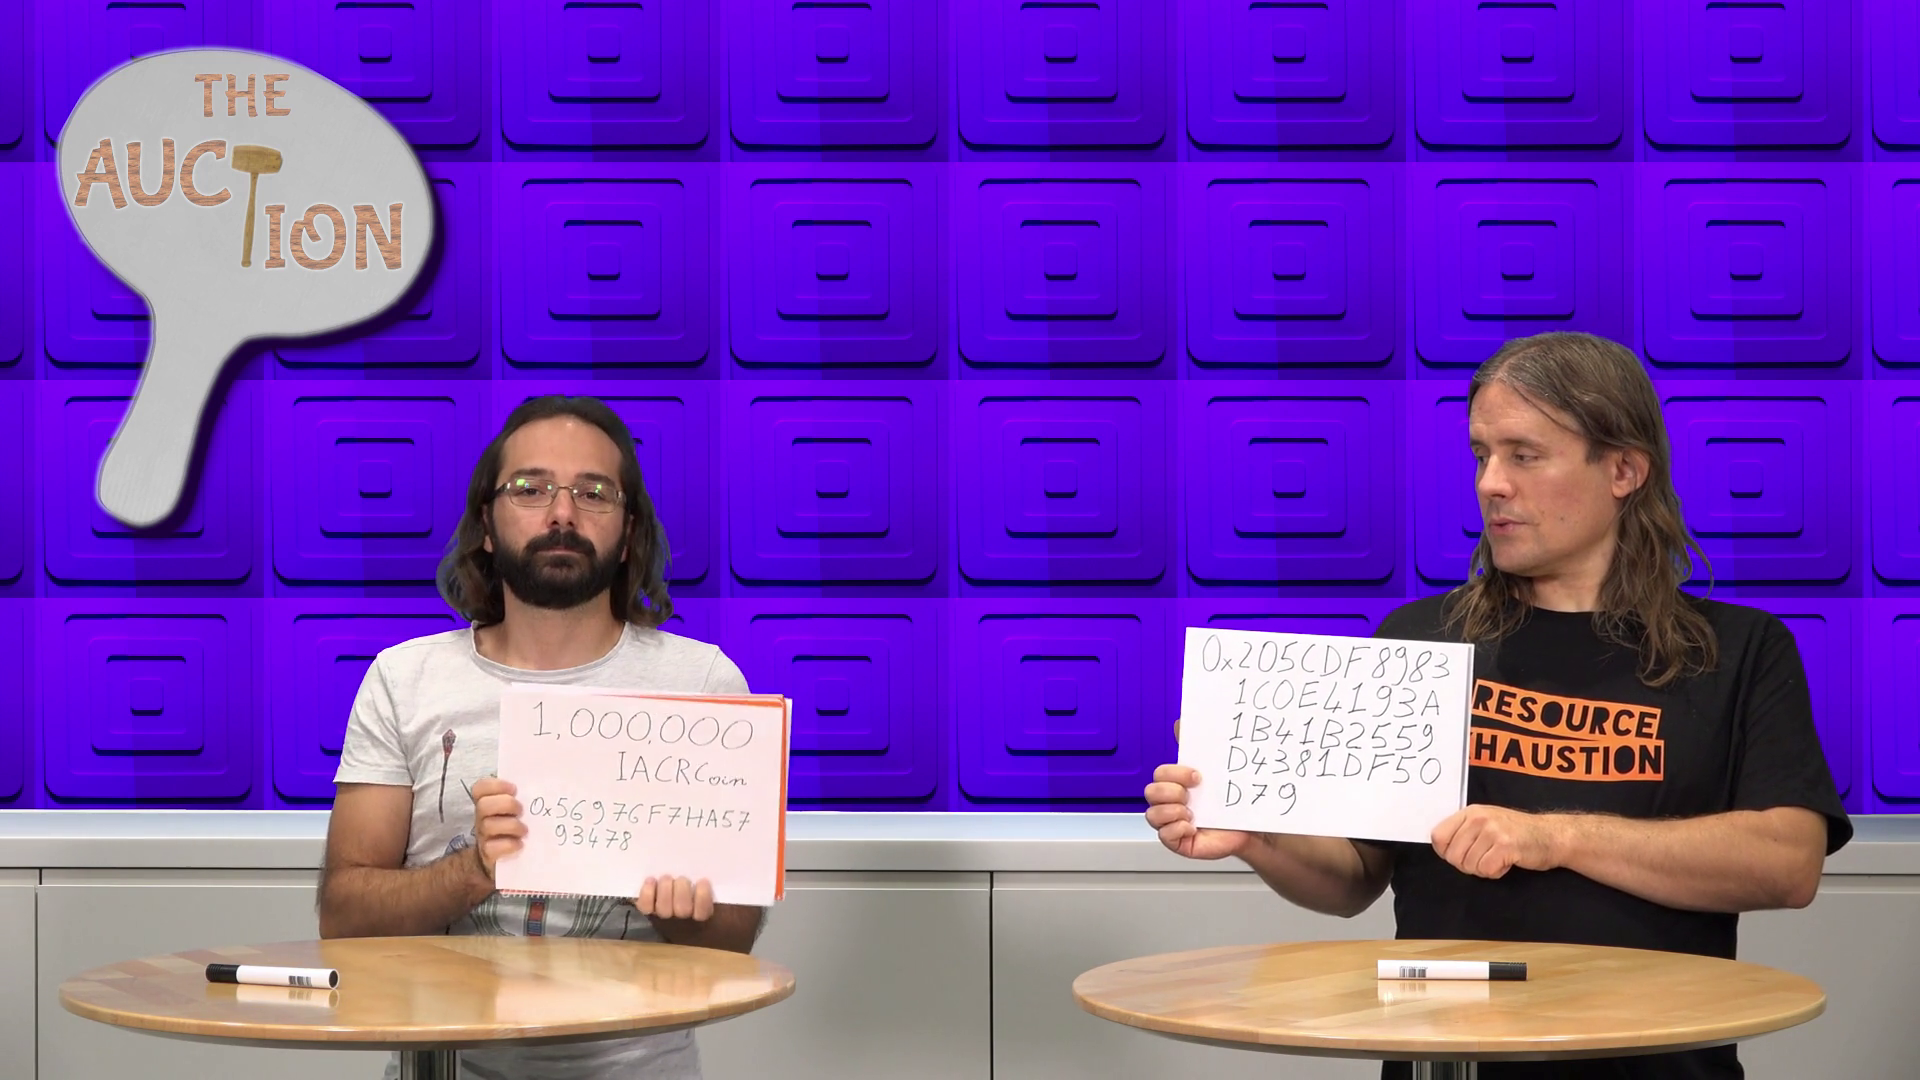
\includegraphics[width=\paperwidth]{reveal.png}
      };
    \end{tikzpicture}
  \end{frame}

  \begin{frame}[plain]
    \begin{tikzpicture}[remember picture,overlay]
      \node(pic)[at=(current page.center)] { 
        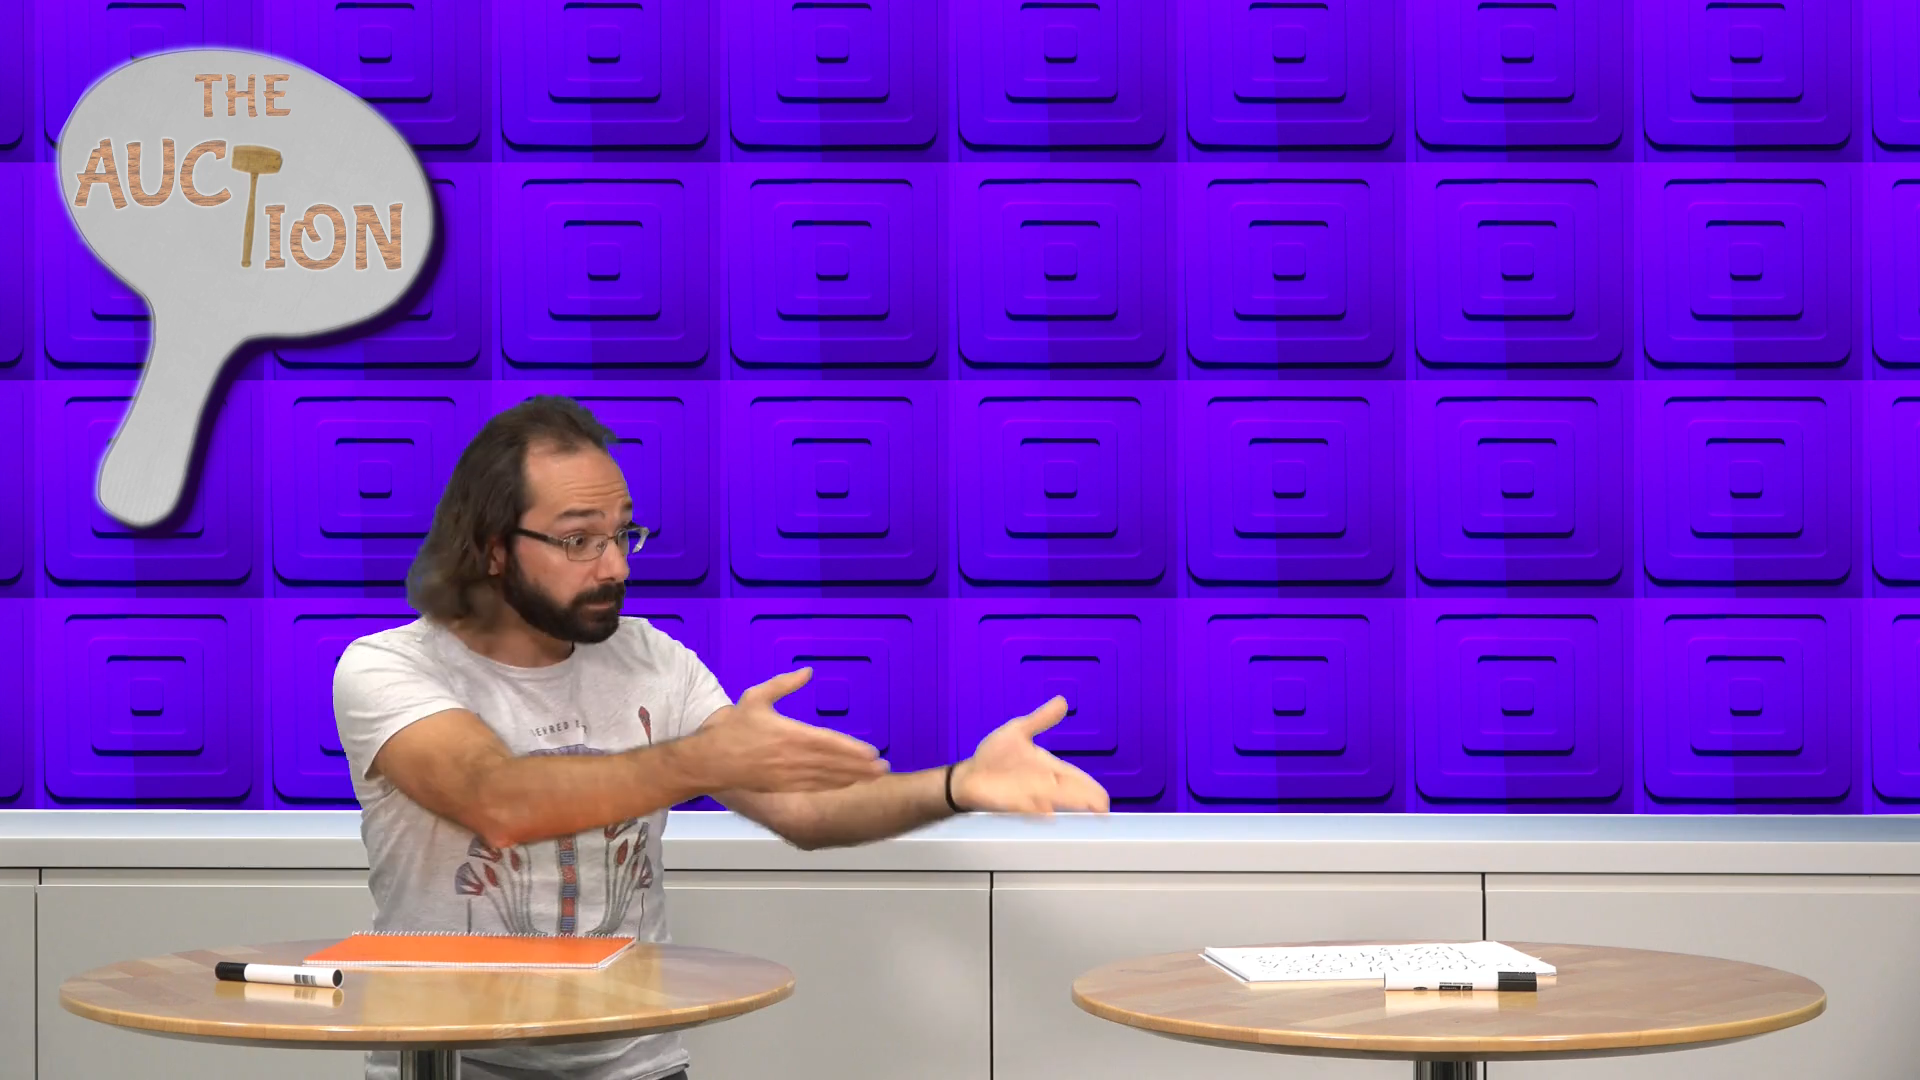
\includegraphics[width=\paperwidth]{complain2.png}
      };
    \end{tikzpicture}
  \end{frame}
}

%%

\begin{frame}{A solution based on TL puzzles}
  \large
  \begin{itemize}
    \setlength{\itemsep}{1.5em}
  \item Each bidder encrypts bid with a TL puzzle;
  \item At the end of the auction each well behaved bidder reveals
    its trapdoor;
  \item Other bids are opened with SlowKDF. \textcolor{gray}{(can
      get quite expensive, though)}
  \end{itemize}
\end{frame}

%%

\begin{frame}{Verifiable Delay Functions (Boneh, Bonneau, Bünz, Fisch 2018)}
  \begin{columns}
    \begin{column}{0.2\textwidth}
      \centering
      \includegraphics[width=0.8\textwidth]{phileas_fogg}

      \vfill

      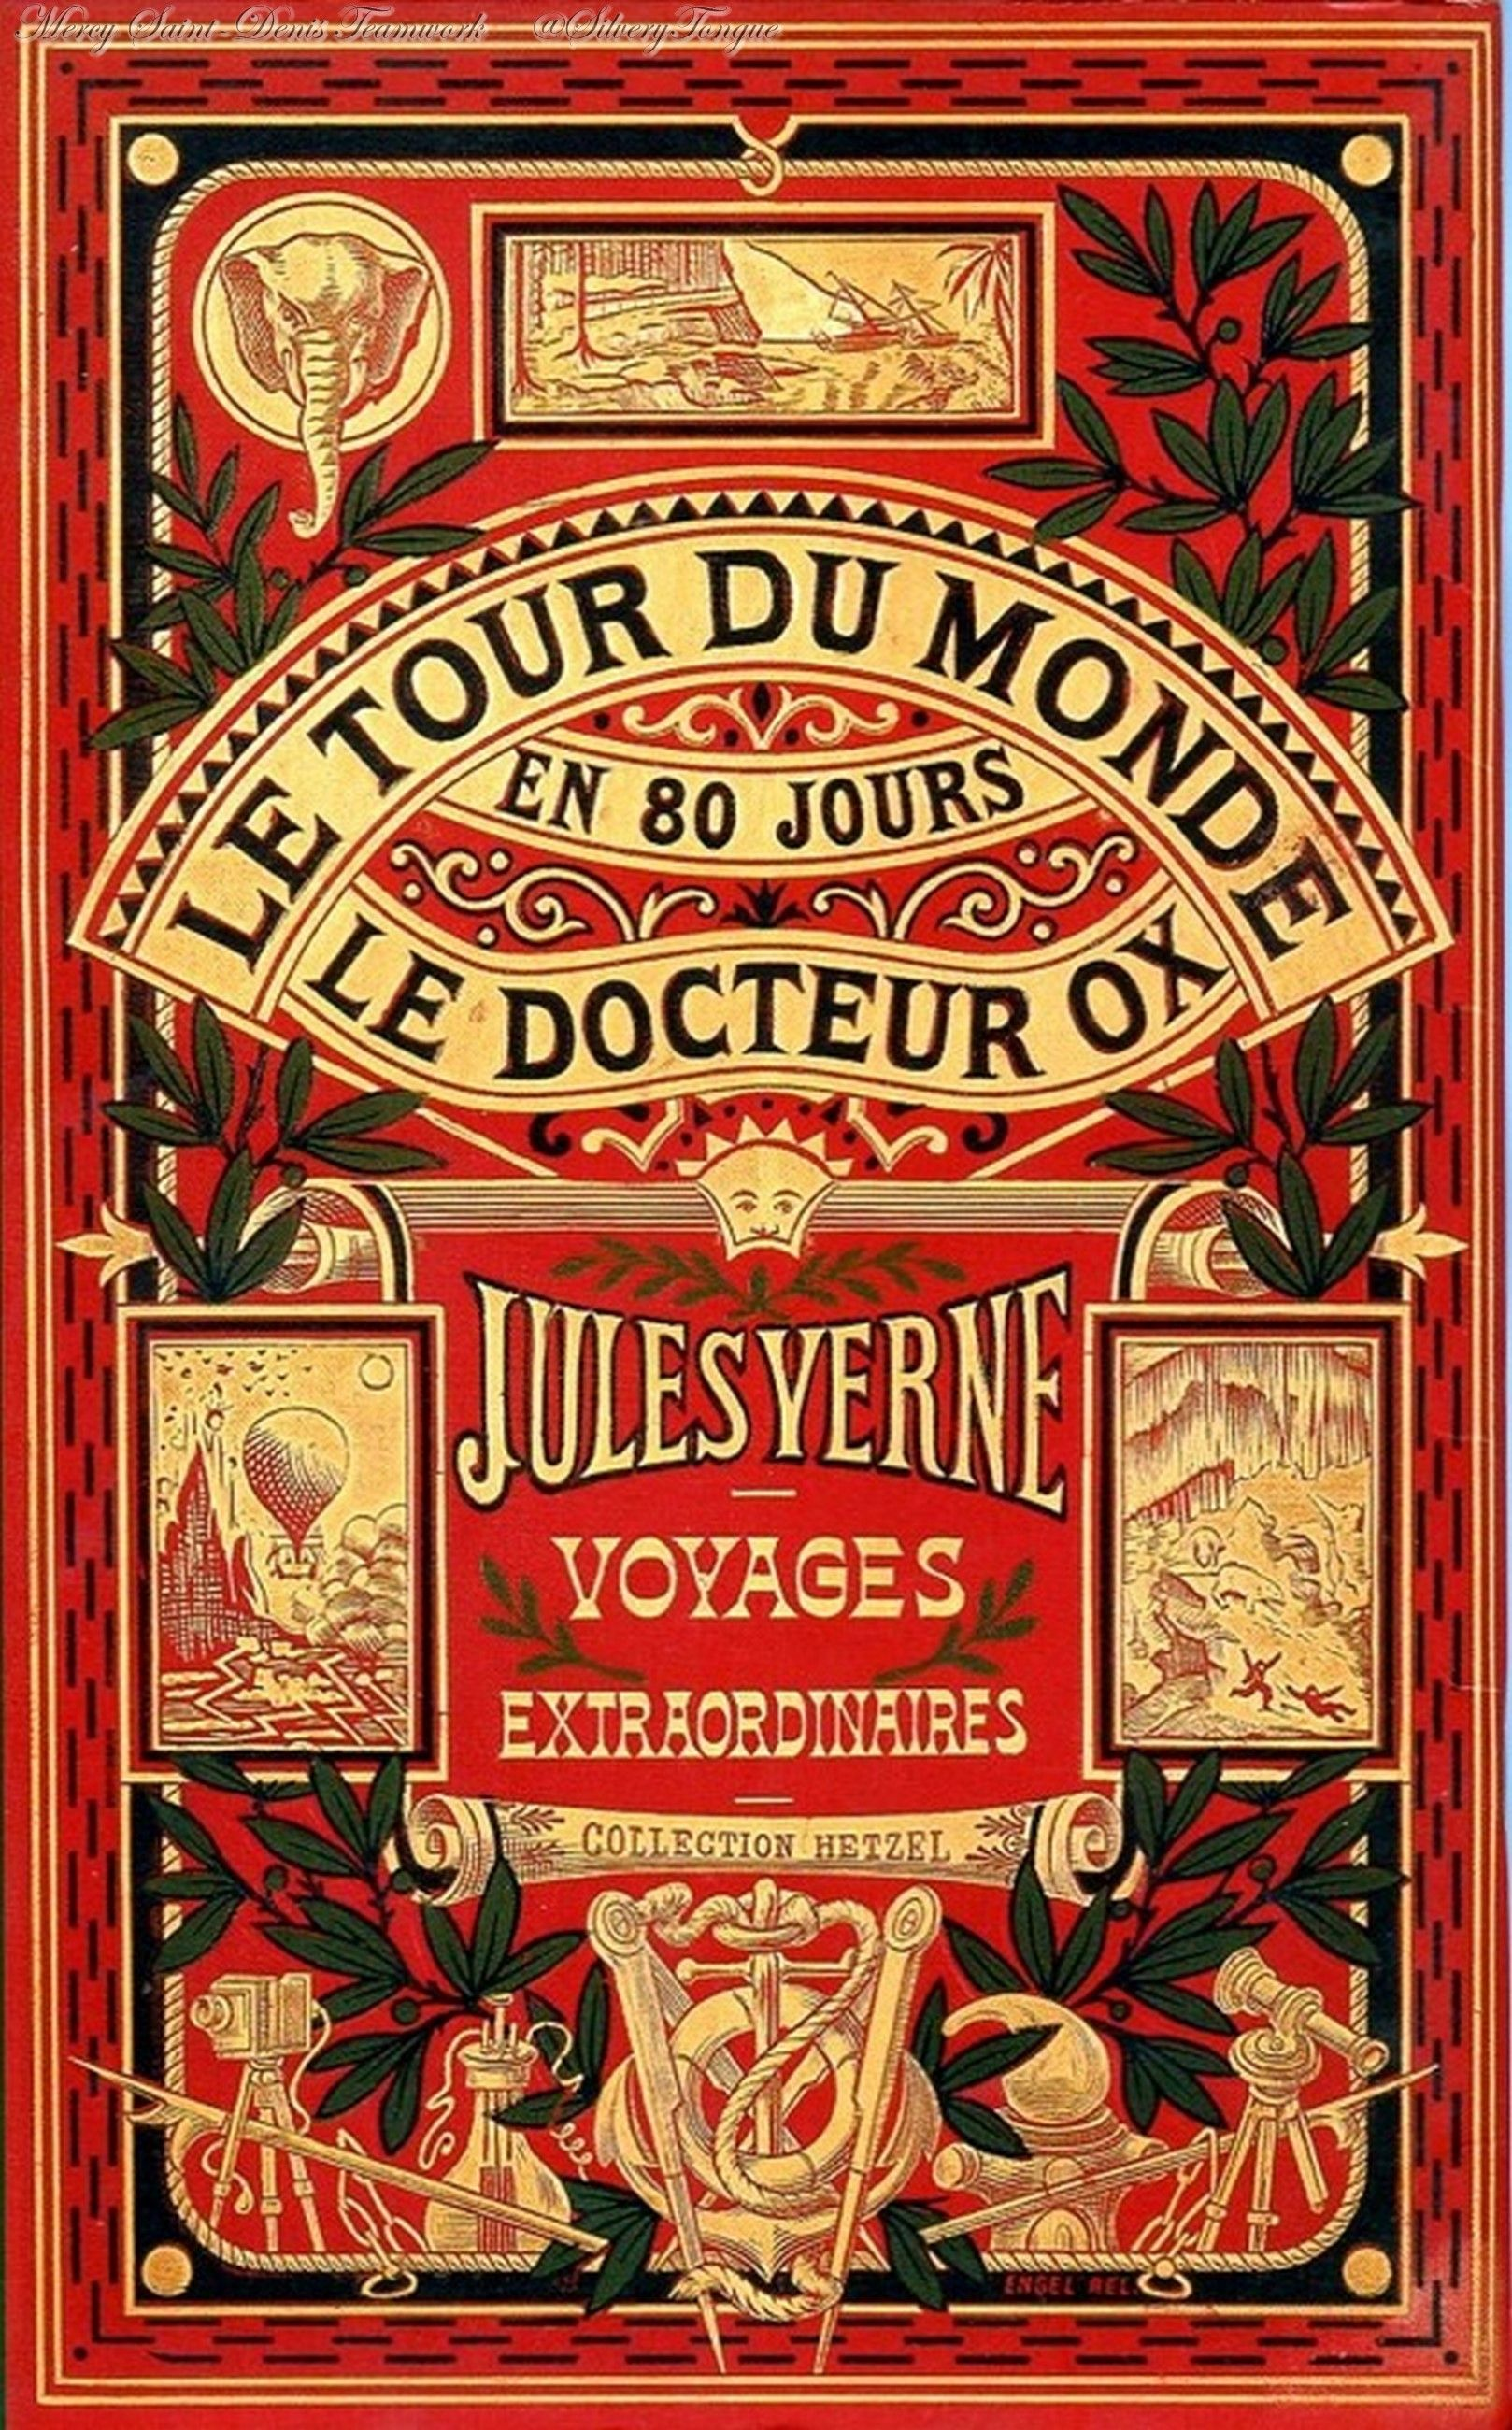
\includegraphics[width=0.8\textwidth]{80jours-couverture}
    \end{column}
    \begin{column}{0.75\textwidth}
      \begin{block}{A sort of \textit{deterministic Proof of Sequential Work}}
        Function (family) \emph{$f:X\to Y$} s.t.:

        \begin{itemize}
        \item Evaluating $f(x)$ takes \emph{long time}:
          \begin{itemize}
          \item \emph{predictably} long time,
          \item on almost all random inputs $x$,
          \item even after having seen many values $f(x')$,
          \item even given \emph{massive number of processors};
          \end{itemize}
        \item Verifying $y=f(x)$ is \emph{efficient}:
          \begin{itemize}
          \item ideally, exponential separation between evaluation and
            verification.
          \end{itemize}
        \end{itemize}
      \end{block}
    \end{column}
  \end{columns}
\end{frame}

%%

\begin{frame}{Example application: distributed lotteries}
  Participants \textbf{A, B, \dots, Z} want to agree on a random
  winning ticket.

  \begin{block}{Flawed protocol}
    \begin{itemize}
    \item Each participant \emph{$x$} broadcasts a random string
      \emph{$s_x$};
    \item Winning ticket is \emph{$H(s_A, \dots, s_Z)$}.
    \end{itemize}

    \pause
    
    Cheating participant \textbf{Z} waits to see all other strings,
    then brute-forces \emph{$s_Z$} to win lottery.
  \end{block}
  
  \pause

  \begin{block}{Fixes}
    \begin{itemize}
    \item Make the hash function \textbf{sloooooooooooooooooooooooooooow};
      \begin{itemize}
      \item e.g., participants have 10 minutes to submit $s_x$,
      \item outcome will be known after 20 minutes.
      \end{itemize}
    \item<4-> Make it possible to verify \emph{$w = H(s_A, \dots, s_Z)$} \textbf{fast}.
    \end{itemize}
  \end{block}
\end{frame}

%%

\begin{frame}{More applications}
  \begin{block}{Randomness beacons}
    \begin{description}
    \item[Goal:] Generate a public stream of provably random numbers.
    \item[Standard technique:] Hash output of public high entropy
      sources (e.g.: stock market, weather, \dots) at regular
      intervals (epochs).
    \item[Risk:] Close to the end of the epoch, adversary manipulates
      the data (e.g., buys stock) repeatedly until they get the
      desired alea.
    \item[Fix:] Run the hashed value through a VDF with delay longer
      than the epoch.
    \end{description}
  \end{block}

  \begin{block}{Proofs of Stake/Space}
    \begin{description}
    \item[Goal:] Elect epoch leader(s) in PoS blockchains.
    \item[Standard technique:] PoS are assigned a ``quality'' (e.g.:
      hash of the PoS), the higher quality gets elected as leader.
    \item[Disadvantage:] Requires synchronization of miners.
    \item[Fix (Chia):] Run the PoS through a VDF with delay
      proportional to quality.
    \end{description}
  \end{block}
\end{frame}

%%

\begin{frame}{Delay Encryption (Burdges and De Feo, 2021)}
  \begin{columns}
    \begin{column}{0.6\textwidth}
      \begin{center}
        \begin{tikzpicture}
          \node (fred) at (0,2) {\includegraphics[height=6em]{fred.png}};
          \node (barney) at (0,0) {\includegraphics[height=6em]{barney.png}};
          \node (scooby) at (3,-2.5) {\includegraphics[height=6em]{scoobydoo.png}};
          \node (jets) at (4,2.2) {\includegraphics[height=7em]{jetsons.png}};
          
          \node (chest) at (6,0) {\includegraphics[width=2em]{chest-closed.png}};
          \node at (6,-1) {\comicneue\bfseries\footnotesize OPEN IN 2112};

          \draw[thick,->] (fred) edge (chest)
          (barney) edge (chest)
          (scooby) edge (chest)
          (jets) edge (chest);
        \end{tikzpicture}
      \end{center}
    \end{column}
    \begin{column}{0.4\textwidth}
      \begin{itemize}
      \item Trapdoor-less time capsule.
      \item Delay Encryption $\Rightarrow$ Time-lock Puzzles.
      \item Delay Encryption $\Rightarrow$ VDF.
      \item Only known from isogenies.
      \item Applications: better auctions, voting, \dots
      \end{itemize}
    \end{column}
  \end{columns}
\end{frame}

%%

\begin{frame}[plain]
  \begin{beamercolorbox}[sep=0.1px,center,wd=\paperwidth,ht=\paperheight]{palette tertiary}
    \begin{columns}
      \begin{column}{0.55\textwidth}
        \Huge\centering Group based\\Delay Functions
      \end{column}
      \begin{column}{0.45\textwidth}
        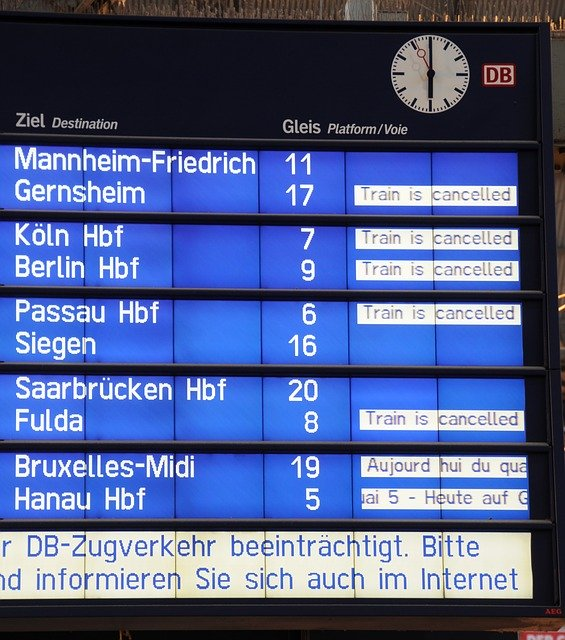
\includegraphics[height=\paperheight]{db.jpg}
      \end{column}
    \end{columns}
  \end{beamercolorbox}
\end{frame}

%%

\begin{frame}[label=current]{Rivest-Shamir-Wagner TL Puzzle ('96)}
  \begin{columns}
    \begin{column}{0.6\textwidth}
      \begin{block}{Setup}
        \emph{$\Z/N\Z$} with $N=pq$ an RSA modulus\\
        $N$ \emph{public}, $p,q$ \emph{private}
      \end{block}

      \begin{block}{Slow KDF}
        With \emph{delay parameter} $\Delta$:
        \begin{align*}
          f:(\Z/N\Z)^\times &\longrightarrow (\Z/N\Z)^\times\\
          x &\longmapsto x^{2^\Delta}
        \end{align*}
        (Conjecturally) takes $\Delta$ squarings.
      \end{block}
    \end{column}
    \begin{column}{0.37\textwidth}
      \centering
      \begin{tikzpicture}[x=2cm,y=2cm]
        \def\crater{29}
        \draw[fill] (360/\crater:1) circle (1pt) +(360/\crater:1em) node {$x$};
        \uncover<2->{
          \draw[fill] (360/\crater : 1) -- (360/\crater*2 : 1)
          circle (1pt) +(360/\crater*2:1em) node {$x^2$};
        }
        \uncover<3->{
          \draw[fill] (360/\crater*2 : 1) -- (360/\crater*3 : 1)
          circle (1pt) +(360/\crater*3:1em) node {$x^4$};
        }
        \uncover<4->{
          \draw[dotted] (360/\crater*3 : 1) arc (360/\crater*3:360/\crater*23:1);
          \draw[fill] (360/\crater*23 : 1) circle (1pt) +(360/\crater*23:1em) node {$x^{2^\Delta}$};
        }
        \uncover<5->{
          \draw[red] (360/\crater : 1) -- node[auto] {$2^\Delta\bmod \varphi(N)$} (360/\crater*23 : 1);
        }
      \end{tikzpicture}

      \medskip
      \uncover<5->{
        \emph{KDF:} knowing $p,q$, we can take a shortcut!
      }
    \end{column}
  \end{columns}
\end{frame}

%%

\begin{frame}{The passage of time}
  Some (problematic?) key assumptions:
  \begin{itemize}
  \item A squaring is a squaring. It cannot possibly go faster than \emph{xxx ns}!
  \item You have a machine that computes a squaring in not much
    more than that!
  \item \emph{$n$ squarings} are $n$ squarings. It cannot take less
    than \emph{$n \times $ one squaring} to do them!
  \item Crucially, even if you have $n$ \emph{parallel processors}!
  \end{itemize}
  These are likely all false, but seem to hold in practice\dots
  
  \medskip\pause

  Some concrete numbers:
  \begin{itemize}
  \item 1 squaring modulo a 2048-bits integer (unknown factorization)
    \begin{itemize}
    \item takes \emph{$\approx 1\mu$s in software};
    \item the current record in \emph{FPGA is 25ns}.
    \end{itemize}
  \item Some example delays:
    \begin{itemize}
    \item 1 hour $\qquad\rightarrow\quad\approx 2^{38}$ squarings,
    \item 1 year $\qquad\rightarrow\quad\approx 2^{51}$ squarings,
    \item 1M years $\quad\rightarrow\quad\approx 2^{71}$ squarings.
    \end{itemize}
  \end{itemize}
\end{frame}

%%

\begin{frame}{Other group based delay primitives}
  \large
  
  \begin{block}{VDFs}
    \begin{itemize}
    \item Pietrzak's proof of evaluation,
    \item Wesolowski's proof of evaluation.
    \end{itemize}
  \end{block}

  \bigskip
  
  \begin{block}{Groups of unknown order}
    \begin{itemize}
    \item RSA groups \textcolor{gray}{$\to$ (trusted setup)}
    \item Class groups of quadratic imaginary fields.
    \end{itemize}
  \end{block}
\end{frame}

%%

\begin{frame}[plain]
  \begin{beamercolorbox}[sep=0.1px,center,wd=\paperwidth,ht=\paperheight]{palette tertiary}
    \begin{columns}
      \begin{column}{0.64\textwidth}
        \Huge\centering Isogeny based\\Delay Functions
      \end{column}
      \begin{column}{0.36\textwidth}
        \includegraphics[height=\paperheight]{phileas_fogg.jpg}
      \end{column}
    \end{columns}
  \end{beamercolorbox}
\end{frame}

%%

\begin{frame}{Elliptic curves and isogenies}
  \begin{columns}
    \begin{column}{0.4\textwidth}
      Elliptic curves
      
      \[y^2 = x^3 + ax + b\]
      
      and their famous \emph{group law}\dots

      \bigskip
      
      \uncover<2->{Isogenies are \emph{morphisms} of elliptic curves.}

      \bigskip
      
      \uncover<3->{\[\frac{\text{Elliptic curves}}{\text{Isogenies}} =
          \frac{\text{Vector spaces}}{\text{Matrices}}\]}
    \end{column}
    \begin{column}{0.6\textwidth}
      \begin{center}
        \begin{tikzpicture}[domain=-2.4566:4,samples=100,yscale=1/2]
          \draw plot (\x,{sqrt(\x*\x*\x-4*\x+5)});
          \draw plot (\x,{-sqrt(\x*\x*\x-4*\x+5)});

          \draw[thin,gray,-latex] (0,-7) -- (0,7);
          \draw[thin,gray,-latex] (-3,0) -- (4,0);
          \draw (-3,1) -- (4,8/3+3);
          \begin{scope}[every node/.style={draw,circle,inner sep=1pt,fill},cm={1,2/3,0,0,(0,3)}]
            \node at (-2.287980,0) {};
            \node at (-0.535051,0) {};
            \node at (3.267475,0) {};
          \end{scope}
          \begin{scope}[every node/.style={yshift=0.3cm},cm={1,2/3,0,0,(0,3)}]
            \node at (-2.287980,0) {$P$};
            \node at (-0.535051,0) {$Q$};
            \node at (3.267475,0) {$R$};
          \end{scope}

          \draw[dashed] (3.267475,3.267475*2/3+3) -- (3.267475,-3.267475*2/3-3) 
          node[draw,circle,inner sep=1pt,fill] {}
          node[xshift=-0.1cm,anchor=east] {$P+Q$};
        \end{tikzpicture}
      \end{center}
    \end{column}
  \end{columns}
\end{frame}

%%

\begin{frame}{Isogenies: an example over $\F_{11}$}
  \centering
  \begin{tikzpicture}[scale=0.4]
    \begin{scope}
      \node[anchor=center] at (0,7) {$E \;:\; y^2 = x^3 + x$};

      \uncover<-1>{
        \draw[thin,gray] (0,-6) -- (0,6);
        \draw[thin,gray] (-6,0) -- (6,0);
      }

      \foreach \x/\y in {0/0,5/3,-4/3,-3/5,-2/1,-1/3} {
        \draw[blue,fill] (\x,\y) circle (0.2) node(E_\x_\y){}
        (\x,-\y) circle (0.2) node(E_\x_-\y){};
      }

      \uncover<2->{\draw[red,fill] (0,0) circle (0.3);}
    \end{scope}

    \draw[black!10!white,thick] (10,-7) -- +(0,14);
    
    \begin{scope}[shift={(20,0)}]
      \node at (0,7) {$E' \;:\; y^2 = x^3 - 4x$};

      \uncover<-1>{
        \draw[thin,gray] (0,-6) -- (0,6);
        \draw[thin,gray] (-6,0) -- (6,0);
      }

      \foreach \x/\y in {0/0,2/0,3/2,4/2,6/4,-2/0,-1/5} {
        \draw[color=blue,fill] (\x,\y) circle (0.2) node(F_\x_\y){}
        (\x,-\y) circle (0.2) node(F_\x_-\y){};
      }
    \end{scope}

    \begin{scope}[color=red,-latex,dashed]
      \begin{uncoverenv}<2->
        \path
        (E_5_3) edge (F_3_2)
        (E_-4_3) edge (F_4_-2)
        (E_-3_5) edge (F_4_2)
        (E_-2_1) edge (F_3_-2)
        (E_-1_3) edge (F_-2_0);
      \end{uncoverenv}
      \begin{uncoverenv}<2->
        \path
        (E_5_-3) edge (F_3_-2)
        (E_-4_-3) edge (F_4_2)
        (E_-3_-5) edge (F_4_-2)
        (E_-2_-1) edge (F_3_2)
        (E_-1_-3) edge (F_-2_0);
      \end{uncoverenv}
    \end{scope}
  \end{tikzpicture}
  
  \begin{columns}
    \begin{column}{0.5\textwidth}
      \[\phi(x,y) = \left(\frac{x^2 + 1}{x},\quad y\frac{x^2-1}{x^2}\right)\]
    \end{column}
    \begin{column}{0.5\textwidth}
      \begin{itemize}
      \item<2-> Kernel generator in \alert{red}.
      \item<2-> This is a degree $2$ map.
      \item<2-> Analogous to $x\mapsto x^2$ in $\F_q^*$.
      \end{itemize}
    \end{column}
  \end{columns}
\end{frame}

%%

\begin{frame}{Up to \emph{isomorphism}}
  \begin{center}
    \begin{tikzpicture}[domain=-2.4566:4,samples=100]
      \newcount\zoomout
      \transduration<15-21>{0.5}
      \animatevalue<15-20>{\zoomout}{0}{10}
      \begin{uncoverenv}<-20>
        \begin{scope}[scale=1-0.09*\zoomout]
          \begin{scope}
            \draw[thin,gray,-latex] (0,-4) -- (0,4);
            \draw[thin,gray,-latex] (-4.2,0) -- (7,0);
          \end{scope}
          
          \newcount\xstretch
          \newcount\ystretch
          \newcount\slant
          \transduration<1-13>{0.5}
          \animatevalue<1-5>{\xstretch}{0}{4}
          \animatevalue<5-9>{\ystretch}{0}{4}
          \animatevalue<9-13>{\slant}{0}{4}      
          \begin{scope}[yscale=0.55-0.05*\the\ystretch,xscale=1+0.1*\the\xstretch,xslant=0.02*\slant]
            \draw plot (\x,{sqrt(\x*\x*\x-4*\x+5)});
            \draw plot (\x,{-sqrt(\x*\x*\x-4*\x+5)});

            \begin{uncoverenv}<-18>
              \draw (-3,1) -- (4,8/3+3);
              \begin{scope}[every node/.style={draw,circle,inner sep=1pt,fill},cm={1,2/3,0,0,(0,3)}]
                \node at (-2.287980,0) {};
                \node at (-0.535051,0) {};
                \node at (3.267475,0) {};
              \end{scope}
              \begin{scope}[every node/.style={yshift=0.3cm},cm={1,2/3,0,0,(0,3)}]
                \node at (-2.287980,0) {$P$};
                \node at (-0.535051,0) {$Q$};
                \node at (3.267475,0) {$R$};
              \end{scope}
              \draw[dashed] (3.267475,3.267475*2/3+3) -- (3.267475,-3.267475*2/3-3) 
              node[draw,circle,inner sep=1pt,fill] {}
              node[xshift=-0.1cm,anchor=east] {$P+Q$};
            \end{uncoverenv}
          \end{scope}

          \begin{uncoverenv}<14>
            \node[anchor=west] at (-4,-3) {\Large\alert{$y^2=x^3+ax+b \quad\longrightarrow\quad j\equiv 1728\frac{4a^3}{4a^3+27b^2}$}};
          \end{uncoverenv}
        \end{scope}
      \end{uncoverenv}
      
      \begin{uncoverenv}<21->
        \draw[fill] (0,0) circle (2pt) node[anchor=north] {$j=1728$};
        \uncover<22>{
          \draw (0.1,0) edge[bend left,->] node[auto] {$\phi$} (7,0);
        }
        \uncover<22->{
          \draw[fill] (7.1,0) circle (2pt) node[anchor=north] {$j=287496$};
        }
        \uncover<23->{
          \draw (0.1,0) edge[bend left,<->,red,very thick] (7,0);
        }
      \end{uncoverenv}
    \end{tikzpicture}
  \end{center}  
\end{frame}

%%

\begin{frame}{The beauty and the beast {\quad\footnotesize(credit: Lorenz Panny)}}
  \begin{overlayarea}{\textwidth}{\textheight}
    \smallskip
    \begin{center}

      Components of particular isogeny graphs look like this:
      \par\vspace{1ex}

      \begin{minipage}{.49\textwidth}\centering
        \begin{tikzpicture}[scale=.6,>=stealth,shorten >=.2mm,shorten <=.2mm,rotate=90,line width=.6pt]
          \isoggraph
        \end{tikzpicture}
      \end{minipage}
      % 
      \begin{minipage}{.49\textwidth}\centering
        \begin{tikzpicture}[scale=2.456,>=stealth,shorten >=.2mm,shorten <=.2mm,rotate=90,line width=.6pt]
          \fpsqgraph
        \end{tikzpicture}
      \end{minipage}

      \only<-2>{
        \vspace{3ex}

        \textit{Which of these is good for VDFs?}
        \pause
        \onslide<2>{%
          \,\textbf{Both!}
        }
      }

    \end{center}
  \end{overlayarea}
\end{frame}

%%

\begin{frame}{Slooooooooooooooooooooooooooooooooooooow isogenies}
  \begin{columns}
    \begin{column}{0.6\textwidth}
      \begin{block}{Setup}
        With \emph{delay parameter} $T$:
        \begin{itemize}
        \item A laaaaaaaaaaaaaaaaaaaaaaaarge isogeny cycle,
        \item<2-> A \emph{starting curve} $E_0$,
        \item<2-> An isogeny \emph{$\phi:E_0\to E_T$} of degree \emph{$2^T$}.
        \end{itemize}
      \end{block}

      \begin{uncoverenv}<3->
        \begin{block}{Evaluation}
          $\phi$ \textbf{is} the VDF:
          \begin{align*}
            \phi:E_0(\F_p) &\longrightarrow E_T(\F_p)\\
            P &\longmapsto \phi(P)
          \end{align*}
          Conjecturally, no faster way than \emph{composing degree $2$
            isogenies}.
        \end{block}
      \end{uncoverenv}
    \end{column}
    \begin{column}{0.37\textwidth}
      \centering
      \begin{tikzpicture}[x=2cm,y=2cm]
        \def\crater{29}
        \draw[fill] (360/\crater:1) circle (1pt) +(360/\crater:1em) node {$E_0$};
        \draw[fill] (360/\crater : 1) -- (360/\crater*2 : 1)
        circle (1pt) +(360/\crater*2:1em) node {$E_1$};
        \draw[fill] (360/\crater*2 : 1) -- (360/\crater*3 : 1)
        circle (1pt) +(360/\crater*3:1em) node {$E_2$};
        \draw[dotted] (360/\crater*3 : 1) arc (360/\crater*3:360/\crater*23:1);
        \draw[fill] (360/\crater*23 : 1) circle (1pt) +(360/\crater*23:1em) node {$E_T$};
        \uncover<4->{
          \draw (0,0) node[anchor=center] {\Large\alert{How to verify?}};
        }
      \end{tikzpicture}
    \end{column}
  \end{columns}  
\end{frame}

%%

\begin{frame}{Isogeny <3 Pairing}
  \begin{block}{Theorem}
    Let \emph{$\phi:E\to E'$} be an isogeny and \emph{$\hat{\phi}:E' \to E$} its dual.
    Let \emph{$e_N$} be the Weil pairing of $E$ and \emph{$e_N'$} that
    of $E'$. %
    Then
    \[e_N(P,\alert{\hat{\phi}}(Q)) = e_N'(\alert{\phi}(P),Q),\]
    for any \emph{$P\in E[N]$} and \emph{$Q\in E'[N]$}.
  \end{block}
  
  \begin{block}{Corollary}
    \[e_N'(\alert{\phi}(P),\alert{\phi}(Q)) = e_N(P,Q)^{\alert{\deg\phi}}.\]
  \end{block}
\end{frame}

%%

\begin{frame}{Isogeny VDF {\small (principle -- De Feo, Masson, Petit and Sanso 2019)}}
  \begin{block}{Setup}
    \begin{itemize}
    \item Pairing friendly curve \emph{$E$},
    \item Isogeny \emph{$\phi:E\to E'$} of degree \emph{$\ell^T$},
    \item Point \emph{$P\in E[N]$}, image \emph{$\phi(P) \in E'[N]$}.
    \end{itemize}
  \end{block}

  \begin{block}{Evaluation}
    \begin{description}
    \item[Input:] random \emph{$Q\in E'[N]$},
    \item[Output:] \emph{$\hat\phi(Q) \in E[N]$}.
    \end{description}
  \end{block}

  \begin{block}{Verification}
    \large
    \[e_N(P,\alert{\hat\phi}(Q)) \quad\overset{?}{=}\quad e_N'(\alert{\phi}(P),Q).\]
  \end{block}
\end{frame}

%% 

\begin{frame}{Comparison}
  \begin{tabular}{l | c c | c c | c c}
    & \multicolumn{2}{c|}{Wesolowski} & \multicolumn{2}{c|}{Pietrzak} & \multicolumn{2}{c}{Ours}\\
    & RSA & class group & RSA & class group & $\F_p$ & $\F_{p^2}$\\
    \hline
    proof size    & $O(1)$ & $O(1)$ & $O(\log(T))$ & $O(\log(T))$ & --- & ---\\
    aggregatable  & yes & yes & yes & yes & --- & ---\\
    watermarkable & yes & yes & yes & yes & (yes) & (yes)\\
    perfect soundness & no & no & no & no & yes & yes\\
    \textit{long} setup & no & no & no & no & \alert{yes} & \alert{yes}\\
    trusted setup & \alert{yes} & no & \alert{yes} & no & \alert{yes} & \alert{yes}\\
    \enskip{}\rotatebox[origin=c]{180}{$\Lsh$} updatable & \alert{no} & --- & \alert{no} & --- & yes & yes\\
    \enskip{}\rotatebox[origin=c]{180}{$\Lsh$} synchronous & \alert{yes} & --- & \alert{yes} & --- & no & no\\
    best attack   & $L_N(1/3)$ & $L_N(1/2)$ & $L_N(1/3)$ & $L_N(1/2)$ & $L_p(1/3)$ & $L_p(1/3)$\\
    quantum annoying & no & (yes) & no & (yes) & no & yes\\
  \end{tabular}
\end{frame}

%%

\begin{frame}
  \centering
  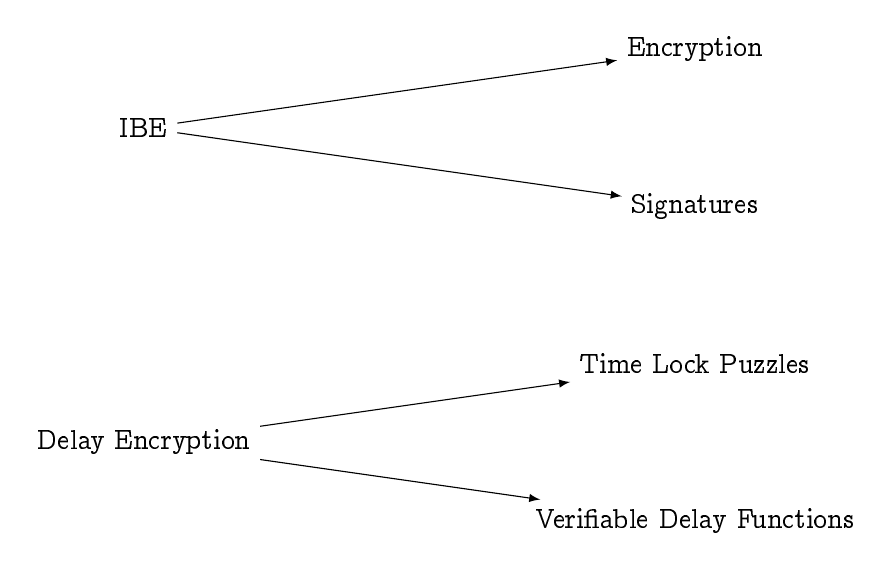
\begin{tikzpicture}
    \node (IBE) at (0,0) {IBE};
    \node (enc) at (7,1) {Encryption};
    \node (sig) at (7,-1) {Signatures};
    \node (DE) at (0,-4) {Delay Encryption};
    \node (TLP) at (7,-3) {Time Lock Puzzles};
    \node (VDF) at (7,-5) {Verifiable Delay Functions};

    \draw[-latex] (IBE) edge (enc) edge (sig)
    (DE) edge (TLP) edge (VDF);
  \end{tikzpicture}
\end{frame}

%%

\begin{frame}{Identity based encryption}
  \centering
  \begin{tikzpicture}
    \begin{scope}[color=white,every node/.style={fill=cyan,inner sep=3mm}]
      \node (keygen) at (0,0) {Keygen};
      \node (encrypt) at (-6,-3) {Encrypt};
      \node (extract) at (6,-3) {Extract};
      \node (decrypt) at (0,-6) {Decrypt};
    \end{scope}

    \begin{scope}
      \node (msk) at (4,-1) {msk};
      \node (pk) at (-4,-1) {pk};
      \node (msg) at (-6,-1) {msg};
      \node (ct) at (-4,-4.5) {ct};
      \node (sk) at (4,-4.5) {sk};
      \node (msg2) at (-6,-6) {msg};
      \node (id) at (0,-3) {
\includegraphics[height=3em]{doge.png}};
      \node[below of=id] {id};
    \end{scope}

    \draw[-latex] (keygen) edge (pk) edge (msk)
    (pk) edge (encrypt)
    (msg) edge (encrypt)
    (encrypt) edge (ct)
    (msk) edge (extract)
    (extract) edge (sk)
    (sk) edge (decrypt)
    (ct) edge (decrypt)
    (decrypt) edge (msg2)
    (id) edge (encrypt) edge (extract);
  \end{tikzpicture}
\end{frame}

%%

\begin{frame}{Boneh--Franklin IBE}
  \centering
  \def\doge{\raisebox{-.6em}{
\includegraphics[height=2em]{doge.png}}}
  \begin{tikzpicture}
    \begin{scope}[color=white,every node/.style={fill=cyan,inner sep=3mm}]
      \node (keygen) at (0,0) {Keygen};
      \node (encrypt) at (-6,-3) {$k = e(u\doge, mG_2)$};
      \node (extract) at (6,-3) {Extract};
      \node (decrypt) at (0,-6) {$k = e(m\doge, uG_2)$};
    \end{scope}

    \begin{scope}
      \node (msk) at (4,-1) {$m$};
      \node (pk) at (-4,-1) {$mG_2$};
      \node (msg) at (-6,-1) {$\mathrm{msg}$};
      \node (ct) at (-4,-5) {$\mathrm{Enc}_k(\mathrm{msg}), uG_2$};
      \node (sk) at (4,-5) {$m\doge$};
      \node (msg2) at (-6,-6) {$\mathrm{msg}$};
      \node (id) at (0,-3) {
\includegraphics[height=3em]{doge.png}};
    \end{scope}

    \draw[-latex] (keygen) edge (pk) edge (msk)
    (pk) edge (encrypt)
    (msg) edge (encrypt)
    (encrypt) edge (ct)
    (msk) edge (extract)
    (extract) edge (sk)
    (sk) edge (decrypt)
    (ct) edge (decrypt)
    (decrypt) edge (msg2)
    (id) edge (encrypt) edge (extract);
  \end{tikzpicture}
\end{frame}

%%

\begin{frame}{Isogeny Based Delay Encryption}
  \centering
  \def\doge{\raisebox{-.6em}{
\includegraphics[height=2em]{doge.png}}}
  \def\iso{\textcolor{red!80!black}{\bm{\phi}}}
  \begin{tikzpicture}
    \begin{scope}[color=white,every node/.style={fill=cyan,inner sep=3mm}]
      \node (keygen) at (0,0) {Setup};
      \node (encrypt) at (-6,-3) {$k = e(u\doge, \iso G_2)$};
      \node (extract) at (6,-3) {Extract};
      \node (decrypt) at (0,-6) {$k = e(\iso\doge, uG_2)$};
    \end{scope}

    \begin{scope}
      \node (msk) at (4,-1) {$\iso$};
      \node (pk) at (-4,-1) {$\iso G_2$};
      \node (msg) at (-6,-1) {$\mathrm{msg}$};
      \node (ct) at (-4,-5) {$\mathrm{Enc}_k(\mathrm{msg}), uG_2$};
      \node (sk) at (4,-5) {$\iso\doge$};
      \node (msg2) at (-6,-6) {$\mathrm{msg}$};
      \node (id) at (0,-3) {
\includegraphics[height=3em]{doge.png}};
    \end{scope}

    \def\clock{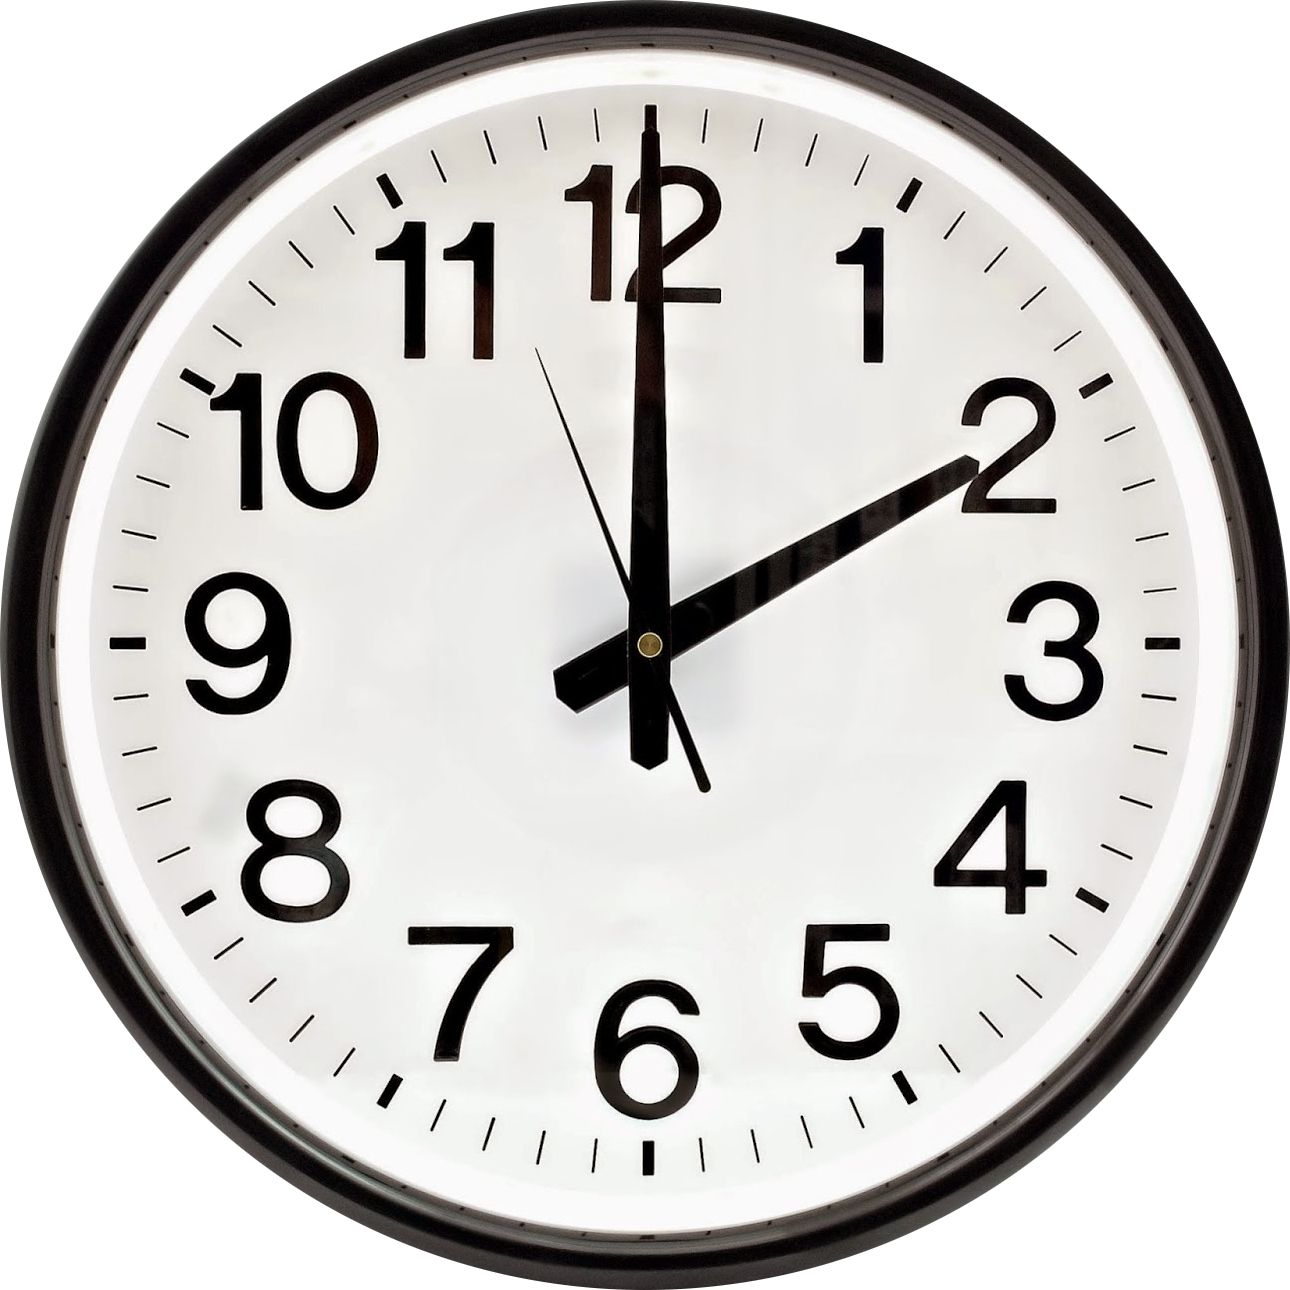
\includegraphics[height=2em]{clock.png}}
    \draw[-latex] (keygen) edge node {\clock} (pk) edge (msk)
    (pk) edge (encrypt)
    (msg) edge (encrypt)
    (encrypt) edge (ct)
    (msk) edge (extract)
    (extract) edge node {\clock} (sk)
    (sk) edge (decrypt)
    (ct) edge (decrypt)
    (decrypt) edge (msg2)
    (id) edge (encrypt) edge (extract);
  \end{tikzpicture}
\end{frame}

%%

\begin{frame}{For concreteness}
  \emph{Elementary step:}
  \medskip
  
  \hspace{2em} RSA: \hfill $x \longmapsto x^2\mod N$ \hspace{4em}

  \vfill
  \hspace{2em} Isogenies: \hfill $\displaystyle x \longmapsto \frac{(x+1)^2}{4\alpha_ix}\mod p$ \hspace{4em}\strut\\
  {\hspace{2em}\normalsize\color{gray} ($\alpha_1,\dots,\alpha_T$ correspond to the isogeny steps)}

  \vfill
  \begin{description}
  \item[Typical parameters:] \emph{$\log_2 p \approx 1500$} gives
    security similar to $\log_2 N \approx 2048$.
  \item[Huge storage:] for a 1 hour delay,
    \begin{itemize}
    \item Isogeny path of length \emph{$\approx 7 \cdot 10^{10}$},
    \item evaluator needs \emph{$\approx$ 16TiB} for storing all
      $(\alpha_1,\dots,\alpha_T)$,
    \item Throughput of \emph{$\approx$ 4.5 GiB/s} to read the
      $\alpha_i$'s from memory.
    \item Storage/speed compromises are available, but it's a tough call!
    \end{itemize}
  \end{description}
\end{frame}

%%

\begin{frame}{(My favorite) open questions}
  \begin{itemize}
  \item Understand the impact of large memory requirements in
    evaluation; is a time/memory trade-off reasonable?
  \item Cryptanalysis, obviously.
  \item Remove trusted setup:
    \begin{itemize}
    \item Hash into the supersingular set, or
    \item Construct ordinary pairing friendly curves with
      exponentially large discriminant.
    \end{itemize}
  \item Explore more advanced pairing+delay constructions.
  \item Spend millions on dedicated hardware for $2$-isogenies.
  \end{itemize}

  \bigskip
  \begin{uncoverenv}<+->
    \begin{center}
      \Large Just Add Isogenies\texttrademark!
    \end{center}
  \end{uncoverenv}
\end{frame}

%%

\def\bl#1{\textcolor{blue}{#1}}
\begin{frame}
  \centering
  \begin{tikzpicture}
    \Large\tt
    \begin{scope}[anchor=west,x=2em]
      \node at (0,0) {\bl{def} extract(x):};
      \node at (1,-1) {\bl{for} i \bl{from} 1 \bl{to} T:};
      \node at (2,-2.5) {$\displaystyle x \leftarrow\frac{(x+1)^2}{4\alpha_i x}$};
      \node at (1,-4) {\bl{return} (x, \textcolor{red}{"Thank You!"})};
    \end{scope}
  \end{tikzpicture}
\end{frame}

\end{document}


% LocalWords:  Isogeny abelian isogenies hyperelliptic supersingular Frobenius
% LocalWords:  isogenous
